%% BEAMER THEME FLIP 2012: Main tex file for compiling
%$ Compile this file. 
%%
%% Copyright 2012 by Flip Tanedo
%% This file may be distributed and/or modified
%% 	1. under the LaTeX Project Public License and/or
%% 	2. under the GNU Public License.
%% 
%% If you e-mail Flip (pt267@cornell.edu) to say that you
%% like this style file, then it would make him smile.

%% Please see notes.txt for comments on Beamer Theme Flip 2013
%% By default, this template is meant to be run with XeLaTeX (for fonts)
%% To run in PDFLaTeX, remove fontspec and any font commands

%% Discussion of Beamer vs XeLaTeX vs LuaLaTeX
%% http://tex.stackexchange.com/questions/29497/xelatex-preventing-beamer-from-using-different-backgrounds

%\def \pgfsysdriver{pgfsys-dvipdfmx.def}

\documentclass[12 pt]{beamer}
\usetheme[
	bullet=circle,		% Other option: square
	bigpagenumber,		% circled page number on lower right
	topline=true,			% colored bar at the top of the frame 
	shadow=false,			% Shading for beamer blocks
	watermark=BG_lower,	% png file for the watermark
	]{Flip}


\newcommand{\titleimage}{title}			% Custom title 
\newcommand{\tanedo}{tanedolight}		% Custom author name
\newcommand{\marilia}{Marília Portela}
\newcommand{\CMSSMDM}{CMSSMDMlight.png}	% light background plot


%%%%%%%%%%
% FONTS %
%%%%%%%%%%

%% Default font: lmodern, doesn't require fontspec % solves some default warnings
\usepackage[T1]{fontenc}
\usepackage{lmodern}			
%\usepackage{sfmath}		% Sans Serif Math, off by default

%% Protects fonts from Beamer screwing with them
%% http://tex.stackexchange.com/questions/10488/force-computer-modern-in-math-mode
\usefonttheme{professionalfonts}


%% XeLaTeX fonts: (comment out if you don't use XeLaTeX)

%% For advanced fonts: access local OS X fonts
\usepackage[no-math]{fontspec}		
%% This template uses typical OS X and Adobe fonts
\defaultfontfeatures{Mapping=tex-text}	% This seems to be important for mapping glyphs properly

%\setmainfont{Gill Sans}			% Beamer ignores "main font" in favor of sans font -- Edição por Marilia : linha comentada 
%\setsansfont{Gill Sans}			% This is the font that beamer will use by default --Edição por Marilia : linha comentada por marilia
% \setmainfont{Gill Sans Light}		% Prettier, but harder to read -- comentada pelo autor do modelo beamer
\usepackage{gillius2}
\setmainfont{Gillius ADF No2}



%\setbeamerfont{title}{family=\fontspec{Gill Sans}}  
\setbeamerfont{title}{family=\fontspec{Gillius ADF No2}} % Edição por Marilia : Substituindo a linha de cima por esta

%\newcommand{\handwriting}{\fontspec{augie}} % From Emerald City, free font
\newcommand{\handwriting}{\fontspec{Augie}} % Edição por Marilia : Substituindo a linha de cima por esta
% \newcommand{\handwriting}{}	% If you prefer no special handwriting font or don't have augie

%\pdfmapfile{=pdftex35.map} % Edição por Marilia  : Não tinha essa linha, eu que coloquei.

%% Gill Sans doesn't look very nice when boldfaced
%% This is a hack to use Helvetica instead
%% Usage: \textbf{\forbold some stuff}
%\newcommand{\forbold}{\fontspec{Helvetica}}
\newcommand{\forbold}{\fontspec{TeX Gyre Heros}} % Edição por Marilia : Substituindo a linha de cima por esta
% \newcommand{\forbold}{} % if you want no special boldface



%%%%%%%%%%%%%%%%%%%%%%%%
% Usual LaTeX Packages %
%%%%%%%%%%%%%%%%%%%%%%%%

\usepackage{amsmath}
\usepackage{amsfonts}
\usepackage{amssymb}
\usepackage{graphicx}
%\usepackage{mathrsfs} 			% For Weinberg-esque letters
%\usepackage{cancel}				% For "SUSY-breaking" symbol
%\usepackage{slashed}            % for slashed characters in math mode
%\usepackage{bbm}                % for \mathbbm{1} (unit matrix)
%\usepackage{amsthm}				% For theorem environment
%\usepackage{multirow}			% For multi row cells in table
%\usepackage{arydshln} 			% For dashed lines in arrays and tables
%\usepackage{tikzfeynman}		% For Feynman diagrams
% \usepackage{subfig}           % for sub figures
% \usepackage{young}			% For Young Tableaux
% \usepackage{xspace}			% For spacing after commands
% \usepackage{wrapfig}			% for Text wrap around figures
% \usepackage{framed}
\usepackage{listings}
%\usepackage{txfonts}
\usepackage[portuguese]{babel}

\newcommand{\heart}{\ensuremath\varheartsuit}


\graphicspath{{images/}}	% Put all images in this directory. Avoids clutter.


\usetikzlibrary{backgrounds}
\usetikzlibrary{mindmap,trees}	% For mind map
% http://www.texample.net/tikz/examples/computer-science-mindmap/


% SOME COMMANDS THAT I FIND HANDY
% \renewcommand{\tilde}{\widetilde} % dinky tildes look silly, dosn't work with fontspec
\newcommand{\comment}[1]{\textcolor{comment}{\footnotesize{#1}\normalsize}} % comment mild
\newcommand{\Comment}[1]{\textcolor{Comment}{\footnotesize{#1}\normalsize}} % comment bold
\newcommand{\COMMENT}[1]{\textcolor{COMMENT}{\footnotesize{#1}\normalsize}} % comment crazy bold
\newcommand{\Alert}[1]{\textcolor{Alert}{#1}} % louder alert
\newcommand{\ALERT}[1]{\textcolor{ALERT}{#1}} % loudest alert
%% "\alert" is already a beamer pre-defined



\author[Marília Portela\quad {marilia.lima@cge.ce.gov.br}]{Marília}
%\title[Flip's Beamer Theme]{Flip's Beamer Theme}
%\institute{Cornell University}
%\date{\today}



\begin{document}

%%%%%%%%%%%%%%%%%%%%%%%%
% Additional  settings %
%%%%%%%%%%%%%%%%%%%%%%%%

%% To use external nodes; http://www.texample.net/tikz/examples/beamer-arrows/
\tikzstyle{every picture}+=[remember picture]


%%%%%%%%%%%%%%%%%%%%%%%%
% Actual content below %
%%%%%%%%%%%%%%%%%%%%%%%%

%% It's much nicer to have all the content in a separate file
\definecolor{gray}{rgb}{0.4,0.4,0.4}
\definecolor{darkblue}{rgb}{0.0,0.0,0.6}
\definecolor{cyan}{rgb}{0.0,0.6,0.6}

\lstset{
  basicstyle=\tiny\ttfamily,
  columns=fullflexible,
  showstringspaces=false,
  commentstyle=\color{jeans}\upshape
}

\newcommand{\functionDefHighlight}[1]{
\bfseries\textcolor{blue}{>} 
%\textcolor{purple}{\mdseries #1}
%\bfseries\textcolor{blue}{<} 
}


\lstdefinelanguage{XML}
{
  morestring=[b]",
  %moredelim=[s][\bfseries\color{blue}]{<}{\ },
  %moredelim=[s][\bfseries\color{blue}]{</}{>},
  %moredelim=[l][\bfseries\color{blue}]{/>},
  %moredelim=[l][\bfseries\color{blue}]{>},
  %moredelim=[s][\bfseries\color{blue}]{>}{<},
  %literate = *{>}{\textcolor{red}>}1
  %  					{<}{\textcolor{red}<}1,
 morecomment=[s]{>}{<},
  morecomment=[s]{<?}{?>},
  stringstyle=\color{crimsonred},
  identifierstyle=\color{blue},
  keywordstyle=\color{cyan},
 %alsoletter={/, </,>},
 alsoletter={', :,<},
  %moredelim=[s][\color{black}]{>}{<},
  ndkeywords={=, <dbms, \'onFail\'},
  morekeywords={
  xmlns, 
  xmlns:xsi,
  xsi:schemaLocation,
  dbms, 
  comments,
  version, 
  file,
  relativeToChangelogFile, 
  type, 
  username,
  id,
  author, onFail,onError,onUpdateSQL,onFailMessage,onErrorMessage, expectedResult, schemaName, tableName, name, columnName, columnNames, viewName,catalogName, foreignKeyName,constraintName,baseColumnNames,baseTableName,referencedColumnNames, referencedTableName,replaceIfExists,primaryKey,nullable,unique, autoIncrement, newColumnName,oldColumnName},
  sensitive=true
}
% DO NOT COMPILE THIS FILE DIRECTLY!
% This is included by the the driver file (FlipBeamerTemplate.tex).

{ %% This is a total kludge for a fancy title page background
\setbeamertemplate{sidebar right}{\llap{
\includegraphics[width=\paperwidth,height=\paperheight]{BG_upper}}}
\begin{frame}[c]%{\phantom{title page}} 
% The \phantom{title page} is a kludge to get the red bar on top
% \titlepage
\begin{center}
	% \includegraphics[width=7cm]{WarpedPenguinsReturn}

	\begin{tikzpicture}%[show background grid] %% Use grid for positioning, then turn off
		\node[inner sep=0pt,above right] (title) 
           { \fontspec{Trebuchet MS}\bfseries \huge LIQUIBASE};
		%	{ \includegraphics[width=7cm]{\titleimage} };
		% \node (title) at (1.5,1.5) {};
	\end{tikzpicture}
	\quad

	% \includegraphics[width=7cm]{\titleimage} 
	
	\vspace{1em}
	\footnotesize\textcolor{gray}{Uma introdução}
	\vspace{.5em}
	
	%\includegraphics[height=1.5cm]{\tanedo} \quad
    {\fontspec{Zapfino Linotype Four} \large Marília Portela} \quad
	% \includegraphics[height=1cm]{FlipSansSerif} \quad
%	\includegraphics[height=1.5cm]{CUasym}\\
	
    
	%\footnotesize\textcolor{gray}{In collaboration with D. Grayson, J. Todd, T. Drake, S. Brown, D. Wayne}\normalsize\\
	\textcolor{normal text.fg!50!Comment}{\textit{CGE},  4 de Setembro de 2017}% \today}
	
\end{center}
\end{frame}
}



\begin{frame}[c]

\begin{block}{Liquibase em três frases}
    \begin{itemize}
        \item Ferramenta de migração de banco de dados
        \item Aplicação stand-alone ou integrada ao projeto java
        \item Atualiza o esquema de qualquer SGBDR suportado
    \end{itemize}
\end{block}

   	\begin{columns}[t]
    \begin{column}[T]{5.5cm}
        \begin{itemize}
            \normalsize
            \item Database.
            \item DB2.	
            \item Derby.	
            \item Firebird.	
            \item H2.	
            \item  HyperSQL.
            \item  Informix.
        \end{itemize}
    \end{column}
    
    \begin{column}[T]{5.5cm}
        \begin{itemize}
             \normalsize
           \item MySQL.
           \item \textcolor{turtlegreen}{Oracle}.
           \item  \textcolor{turtlegreen}{PostgreSQL}.
           \item SQL Server.
           \item SQLite.
           \item Sybase.
           \item Sybase Anywhere.
       \end{itemize}
    \end{column}
\end{columns}

\end{frame}

\begin{frame}[fragile]{Changelog - o coração do liquibase}
%\heart o coração do liquibase
\begin{itemize}
    \small \item Define operação principal do liquibase.
    \small \item Pode conter um ou mais changesets (unidades de mudança).
    \small \item Geralmente inclui outros changelogs, gerando uma hierarquia de arquivos
\end{itemize}
\begin{block}{db.changelog-master.xml}
 \begin{lstlisting}[language=XML]
        <databaseChangeLog
            xmlns="http://www.liquibase.org/xml/ns/dbchangelog/1.8"
            xmlns:xsi="http://www.w3.org/2001/XMLSchema-instance"
            xsi:schemaLocation="http://www.liquibase.org/xml/ns/dbchangelog/1.8
            http://www.liquibase.org/xml/ns/dbchangelog/dbchangelog-1.8.xsd">  
            
            <include file="db.changelog-1.0.xml" relativeToChangelogFile="true" />
            <include file="db.changelog-2.0.xml" relativeToChangelogFile="true" />
        
        </databaseChangeLog>
\end{lstlisting}
\end{block}
\end{frame}

\begin{frame}[fragile]{Changelog - o coração do liquibase}
    
\begin{columns}[t]
  \begin{column}[T]{2cm}
    \begin{itemize}
        \normalsize
        \item \only<1>{\textcolor{ALERT}}{XML}.
        \item \only<2>{\textcolor{ALERT}}{SQL}.
        \item JSON.
        \item YAML.
        \item Groovy.
    \end{itemize}
 \end{column}
  \begin{column}[T]{9cm}
  %  \begin{overlayarea} Exemplo:
    \begin{onlyenv}<1>
    \begin{lstlisting}[language=XML]
    <databaseChangeLog
        xmlns="http://www.liquibase.org/xml/ns/dbchangelog/1.8"
        xmlns:xsi="http://www.w3.org/2001/XMLSchema-instance"
        xsi:schemaLocation="http://www.liquibase.org/xml/ns/dbchangelog/1.8
        http://www.liquibase.org/xml/ns/dbchangelog/dbchangelog-1.8.xsd">
        
        <changeSet id="1" author="marilia">
            <addColumn catalogName="cat" schemaName="public"  tableName="carro">
                <column name="modelo" type="varchar(255)"/>
            </addColumn>
        </changeSet>
        
        <changeSet id="2" author="bob">
            <renameColumn   oldColumnName="modelo" 
                                       newColumnName="tipo" tableName="carro" />
        </changeSet>
    
    </databaseChangeLog>
    \end{lstlisting}
\end{onlyenv}
    \begin{onlyenv}<2>
        \begin{lstlisting}[language=SQL]
            --liquibase formatted sql
            
            --changeset nvoxland:1
            create table test1 (
            id int primary key,
            name varchar(255)
            );
            --rollback drop table test1;
            
            --changeset nvoxland:2
            insert into test1 (id, name) values (1, ‘name 1′);
            insert into test1 (id, name) values (2, ‘name 2′);
            
            --changeset nvoxland:3 dbms:oracle
            create sequence seq_test;
        \end{lstlisting}
\end{onlyenv}
%\end{overlayarea}
\end{column}
\end{columns}

\end{frame}

\begin{frame}[c]{Aborgadem Geral}
\begin{itemize}
        \item Liquibase cria e mantém a tabela DATABASECHANGELOG que registra todas as mudanças executadas. Sempre que executa, ele a verifica para não reaplicar os mesmos changesets.
        \item A tabela DATABASECHANGELOCK também é criada e gerenciada pelo Liquibase para fins de controle de concorrência.
\end{itemize}

\begin{center}
\begin{tikzpicture}
\node[inner sep=0pt,above right] (title) 
{ 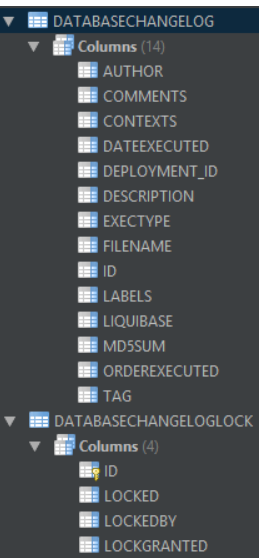
\includegraphics[scale=0.35]{databasechangelog} };
\end{tikzpicture}
\end{center}
\end{frame}

\begin{frame}[c]{Aborgadem Geral}
\begin{itemize}
    \item Mudanças descritas de forma estritamente incremental.
    \item Quando uma mudança (changeset) é introduzida no changelog (e potencialmente executada no BD), \textcolor{ALERT}{ela não deve ser alterada.}
\end{itemize}
\begin{center}
     \begin{tikzpicture}
    \node[inner sep=0pt,above right] (title) 
    { 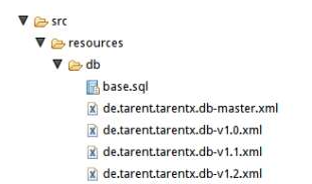
\includegraphics[scale=0.60]{screenshot001} };
    \end{tikzpicture}  
\end{center}
\end{frame}

\begin{frame}[c]{Execução}
\begin{itemize}
    \item Gradle.
    \item Maven.
    \item Software CI.
    \item \textcolor{ALERT}{ServletListener}.
    \item \textcolor{ALERT}{Linha de comando com a aplicação stand-alone}.
\end{itemize}
\begin{center}
    \begin{tikzpicture}
    \node[inner sep=0pt,above right] (title) 
    { 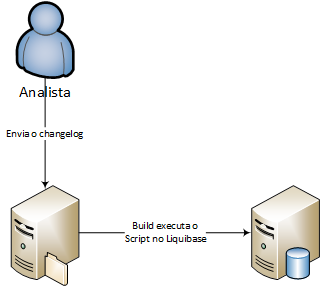
\includegraphics[scale=0.65]{Imagem1} };
    \end{tikzpicture}  
\end{center}

\end{frame}

\begin{frame}[fragile]{Execução}{Configuração ServletListener}
\begin{block}{Arquivo web.xml}
%\begin{center}
    \begin{lstlisting}[language=XML]
    <context-param>
        <param-name>liquibase.changelog</param-name>
        <param-value>/liquibase/changelog/db.changelog-master.xml</param-value>
    </context-param>
    
    <context-param>
        <param-name>liquibase.datasource</param-name>
        <param-value>java:/liquibaseDS</param-value>
    </context-param>
    
    <context-param>
        <param-name>liquibase.host.includes</param-name>
        <param-value>
                               localhost,
                               e-parceriashomol.cge.local,
                               e-parceriasdesenv.cge.local,
                               e-parceriashomol2.cge.local
         </param-value>
    </context-param>
    
    <listener>
        <listener-class>liquibase.integration.servlet.LiquibaseServletListener</listener-class>
    </listener>
    \end{lstlisting}
%\end{center}
\end{block}

\tiny *Já que o usuário do banco de dados configurado para o liquibase precisa ter permissões de criação de objetos de BD, é aconselhável criar um datasource (liquibaseDS) diferente do usado pela aplicação.

\end{frame}

\begin{frame}[c]{Execução}{Configuração Linha de Comando}

\begin{block}{liquibase.properties}
    changeLogFile=changelog-master.xml
    
    driver: org.hsqldb.jdbc.JDBCDriver
    
    classpath: D:/Tools/HSQLDB/hsqldb-2.3.1/hsqldb/lib/hsqldb.jar
    
    url: jdbc:hsqldb:hsql://localhost/teste-liquibase-s
    
    username: root 
    
    password: root
\end{block}

\tiny *Note os caminhos são relativos ao diretório atual.

\tiny **Liquibase procura o arquivo liquibase.properties no diretório atual, ou no caminho provido na opção --defaultsFile do comando liquibase
\end{frame}

\begin{frame}[c]{Execução}{Usando a Linha de Comando}

\begin{block}{Criando tag e voltando ao ponto da tag}
    liquibase tag “tag1”
    
    liquibase update
    
    liquibase rollback “tag1”
\end{block}

\begin{block}{Gerando documentação sobre as mudanças}
    liquibase dbdoc documentacao
\end{block}
\begin{center}
    \begin{tikzpicture}
    \node[inner sep=0pt,above right] (title) 
    { 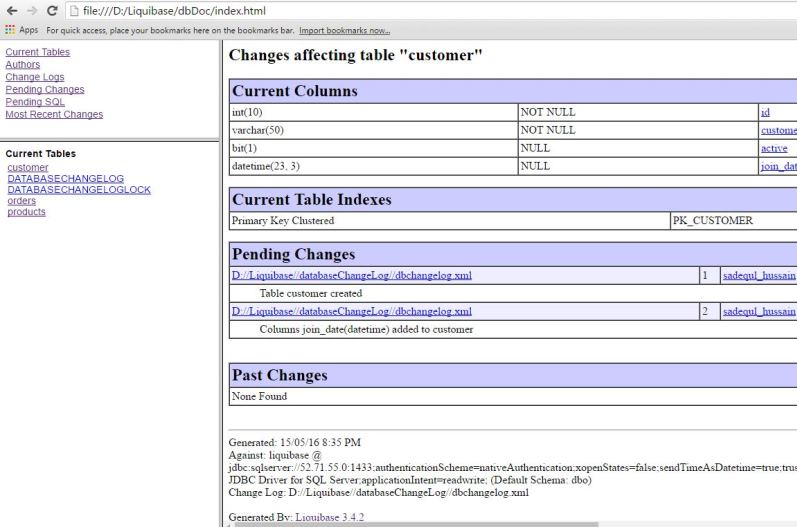
\includegraphics[scale=0.45]{documentacao} };
    \end{tikzpicture}  
\end{center}

\end{frame}

\begin{frame}[fragile]{Refatorações(DDLs)}
\begin{block}{Criação de Tabelas}
    \begin{lstlisting}[language=XML]               
        <changeSet id="1" author="marilia">
        
            <createTable tableName="tabelaA">
                <column name="id" type="bigint" autoIncrement="true">
                    <constraints primaryKey="true" nullable="false"/>
                </column>
                <column name="codigo" type="varchar(20)">
                    <constraints nullable="false" unique="true"/>
                </column>
                <column name="descricao" type="varchar(200)"/>
            </createTable>
            
            <addUniqueConstraint columnNames="codigo,descricao"
                constraintName="codigo_desc" tableName="tabelaA"/>
            
            <createTable tableName="tabelaB">
                <column name="id" type="bigint" autoIncrement="true">
                    <constraints primaryKey="true" nullable="false"/>
                </column>
                <column name="id_tabelaA" type="bigint"/>
            </createTable>
            
            <addForeignKeyConstraint baseColumnNames="id_tabelaA" baseTableName="tabelaB" 
              referencedColumnNames="id" referencedTableName="tabelaA" constraintName="id_tabelaA_fk"/>
              
        </changeSet>
    \end{lstlisting}
\end{block}
\end{frame}

\begin{frame}[fragile]{Refatorações(DDLs)}
O liquibase é capaz de gerar o rollback do changeset automaticamente, com exceção de alguns casos especiais, nos quais ele deve ser explicitamente descrito.
\begin{block}{Rollbacks}
    \begin{lstlisting}[language=XML]
    <databaseChangeLog
    xmlns="http://www.liquibase.org/xml/ns/dbchangelog/1.8"
    xmlns:xsi="http://www.w3.org/2001/XMLSchema-instance"
    xsi:schemaLocation="http://www.liquibase.org/xml/ns/dbchangelog/1.8
    http://www.liquibase.org/xml/ns/dbchangelog/dbchangelog-1.8.xsd">
    
        <changeSet id="1" author="marilia">
            <dropTable tableName="nomeTabela"/>
            <rollback>
                <createTable tableName="nomeTabela">
                    <column name="id" type="int"/>
                </createTable>
            </rollback>
        </changeSet>
    </databaseChangeLog>
    \end{lstlisting}
\end{block}
\end{frame}

\begin{frame}[fragile]{Refatorações(DDLs)}
\begin{block}{Criação de Views}
    \begin{lstlisting}[language=XML]
    <databaseChangeLog
        xmlns="http://www.liquibase.org/xml/ns/dbchangelog/1.8"
        xmlns:xsi="http://www.w3.org/2001/XMLSchema-instance"
        xsi:schemaLocation="http://www.liquibase.org/xml/ns/dbchangelog/1.8
        http://www.liquibase.org/xml/ns/dbchangelog/dbchangelog-1.8.xsd">
        
        <changeSet id="1" author="marilia">
            <createView catalogName="cat" schemaName="public"  viewName="vi_pessoa"
                               replaceIfExists="true">
                SELECT id, name FROM pessoa WHERE id > 10
            </createView>
        </changeSet>
         
    </databaseChangeLog>
    \end{lstlisting}
\end{block}
\end{frame}

\begin{frame}[fragile]{Refatorações(DDLs)}
\begin{block}{Criação de Procedures e Triggers}
    \begin{lstlisting}[language=XML]
        <changeSet id="1" author="marilia">
            <createProcedure comments="Um comentário" dbms="postgreSQL">
                CREATE OR REPLACE FUNCTION change_update_time() RETURNS trigger
                LANGUAGE plpgsql
                AS $$
                BEGIN
                NEW.updated_at := CURRENT_TIMESTAMP;
                RETURN NEW;
                END;
                $$;
            </createProcedure>
            <rollback>
                DROP FUNCTION change_update_time();
            </rollback>
        </changeSet>
        
        <changeSet id="2" author="marilia">
            <sql dbms="postgreSQL">
                DROP TRIGGER IF EXISTS trigger_auditoria ON tabelaA;
                CREATE TRIGGER trigger_auditoria 
                BEFORE UPDATE ON tabelaA 
                FOR EACH ROW EXECUTE PROCEDURE change_update_time();
            </sql>
            <rollback>
                DROP TRIGGER trigger_auditoria ON tabelaA;
            </rollback>
        </changeSet>
    \end{lstlisting}
\end{block}
\end{frame}

\begin{frame}[fragile]{Refatorações(DDLs)}

\begin{block}{Pré-condições}
    \begin{lstlisting}[language=XML]
    <databaseChangeLog
        xmlns="http://www.liquibase.org/xml/ns/dbchangelog/1.8"
        xmlns:xsi="http://www.w3.org/2001/XMLSchema-instance"
        xsi:schemaLocation="http://www.liquibase.org/xml/ns/dbchangelog/1.8
        http://www.liquibase.org/xml/ns/dbchangelog/dbchangelog-1.8.xsd">
        <preConditions>
            <dbms type="oracle" />
            <runningAs username="SYSTEM" />
        </preConditions>

        <changeSet id="1" author="marilia">
            <preConditions onFail="WARN">
                <sqlCheck expectedResult="0">select count(*) from tabelaVelha</sqlCheck>
            </preConditions>
            <comment>
                    Comentários vêm depois da pré-condição.  
                    Do contrário, liquibase mostra um erro.
                    'onFail' e 'onError' admitem os atributos: HALT(default), CONTINUE, MARK_RUN e WARN
            </comment>
            <dropTable tableName="tabelaVelha"/>
        </changeSet>
    </databaseChangeLog>
    \end{lstlisting}
\end{block}
\end{frame}


\begin{frame}[fragile]{Carregando Dados}
\begin{onlyenv}<1> 
\begin{block}{Insert}
    \begin{lstlisting}[language=XML]
    <changeSet id="2" author="marilia">
        <insert schemaName="nome-esquema" tableName="tabelaB">
            <column name="descricao">O registro foi finalizado</column>
            <column name="id_tabelaA">
                (SELECT id FROM tabelaA WHERE codigo='FINALIZADO')
            </column>
        </insert>
    </changeSet>
    \end{lstlisting}
\end{block}
\end{onlyenv}
\begin{onlyenv}<2>
\begin{block}{Load}
    \begin{lstlisting}[language=XML]
        <changeSet id="2" author="marilia">
            <loadData file="db.changelogs/dados.csv"
                schemaName="nome_esquema" quotchar="'" tableName="tabelaA"/>
        </changeSet>
    \end{lstlisting}
\end{block}
\normalsize \textcolor{jeans}{dados.csv} \\
\tiny \textbf{Codigo,Descricao} \\
\tiny 'EFETIVADO','Item finalizado' \\
\tiny 'AUTORIZADO','Item autorizado' \\
\tiny 'CANCELADO','Item Cancelado' \\
\end{onlyenv}
\end{frame}

\begin{frame}[c]{Mais Informações}
\only<1>{
\textit{Links:} 

\href{http://www.liquibase.org/bestpractices.html}{Melhores práticas}

\href{http://www.liquibase.org/documentation/changes}{Sintax nos changelogs}

\href{http://www.liquibase.org/documentation/update.html}{Atualização}

\href{http://www.liquibase.org/documentation/command_line.html}{Linha de comando}
}
\only<2>{
\begin{tikzpicture}
\node[inner sep=0pt,below right] (title) 
{ \fontspec{Trebuchet MS}\bfseries \huge DEMONSTRAÇÃO};
\end{tikzpicture}
}
\end{frame}



% \begin{frame}{test}
% 	Main text still in Gill Sans
% 	$$\frac{f}{f^4}$$
% 	
% 	But math is now different
% 	\Large
% 	$$\frac{f^2}{f^4}$$
% \end{frame}


\end{document}

